\documentclass{article}

\usepackage{amsmath}
\usepackage{amssymb}
\usepackage{cleveref}
\usepackage{fullpage}
\usepackage{graphicx}

\newcommand{\RR}{\mathbb{R}}
\newcommand{\sample}[1]{#1^{[s]}}
\newcommand{\ep}{\varepsilon}

\begin{document}
	
\section{Standard Gaussian Process Fitting}

Suppose we have a vector of output variables $y\in\RR^N$, with associated matrix of input variables $X\in\RR^{N\times k}$. Note that $N$ represents the number of observations and $k$ represents the number of input variables. Suppose there is a true relationship between $y$ and $X$ given by $y = f(X)$, where the function $f$ is unknown to the researcher. Gaussian processes aim to approximate $f$ via the following model:

\begin{subequations}
\begin{align}
	\label{eq:GPBase:theta} \theta &\sim g_\theta(\phi_\theta)\\ 
	\label{eq:GPBase:sigma} \sigma &\sim g_\sigma(\phi_\sigma)\\ 
	\label{eq:GPBase:f} f(X) &\sim N(0, K_\theta(X))\\ 
	\label{eq:GPBase:y} y &\sim N(f(X), \sigma^2 I_N). 
\end{align}
\end{subequations}

\noindent \Cref{eq:GPBase:theta} and \cref{eq:GPBase:sigma} represent priors over parameters $\theta$ and $\sigma$. \Cref{eq:GPBase:f} is the prior over values of $f(X)$, formed using kernel function $K_\theta$. A common choice of kernel function is the normal kernel, also referred to as the exponentiated quadratic kernel. This kernel function takes the form

\begin{equation}
	K_\theta(X)_{ij} = \alpha^2 \exp\left(-\frac12 (X_i - X_j)' P^{-1} (X_i - X_j)\right)\mbox{\ \ \ \ }\forall i=1,...,N; j=1,...,N,
\end{equation}

\noindent where $\alpha$ is a positive scalar, $P$ is a positive definite $k\times k$ matrix, and $X_i\in\RR^k$ is the $i$th row of $X$. This implies that $K := K_\theta(X)$ is an $N\times N$ positive definite matrix. Finally, \cref{eq:GPBase:y} relates observations of output, $y$, to their predicted values, $f(X)$.

The above form presents difficulties in sampling for a couple of reasons. First, $f$ has a strong prior dependence on kernel parameters $\theta$ in \cref{eq:GPBase:f} that can lead to inefficient sampling (Betancourt and Girolami 2013). To reduce this prior dependence, first denote the Cholesky decomposition of $K$ as $K = LL'$. Then, we can rewrite the model as 

\begin{subequations}
\begin{align}
	\label{eq:GPChol:theta} \theta &\sim g_\theta(\phi_\theta)\\ 
	\label{eq:GPChol:sigma} \sigma &\sim g_\sigma(\phi_\sigma)\\ 
	\label{eq:GPChol:eta} \eta &\sim N(0, I_N)\\
	\label{eq:GPChol:K} K_\theta(X) &= LL'\\
	\label{eq:GPChol:f} f(X) &= L\eta\\ 
	\label{eq:GPChol:y} y &\sim N(f(X), \sigma^2 I_N). 
\end{align}
\end{subequations}

\noindent This model is equivalent to the one presented above by properties of multiplying a normally-distributed random variable by a constant matrix, which imply that

\begin{subequations}
\begin{align}
	f(X) = L\eta &\sim N(L\times E[\eta], L\times \mbox{var}(\eta)\times L')\\ 
	&\equiv N(L\times 0, L\times I_N \times L')\\ 
	&\equiv N(0, K).
\end{align}
\end{subequations}

This form still presents difficulties in sampling because its posterior distribution is of high dimensionality; using a normal kernel, there are $N + 3$ parameters to sample. We can note, however, that

\begin{equation}
	f(X) \sim N(0, K_\theta(X))
\end{equation}

\noindent and

\begin{equation}
	y \sim N(f(X), \sigma^2 I_N),
\end{equation}

\noindent imply that

\begin{equation}
	y \sim N(0, K_\theta(X) + \sigma^2 I_N).
\end{equation}

\noindent Altogether, the model becomes

\begin{subequations}
\begin{align}
	\label{eq:GPFinal:theta} \theta &\sim g_\theta(\phi_\theta)\\ 
	\label{eq:GPFinal:sigma} \sigma &\sim g_\sigma(\phi_\sigma)\\ 
	\label{eq:GPFinal:y} y &\sim N(0, K_\theta(X) + \sigma^2 I_N). 
\end{align}
\end{subequations}

This model only requires sampling of $\theta$ and $\sigma$, greatly reducing the dimensionality of the model. Further, the mean and variance of $y|f(X)$ can still be derived, described in more detail in the following section.

\section{Standard Gaussian Process Inference}

Suppose that we have drawn $S$ samples of $\theta$ and $\sigma$ from their posterior distributions. Denote the $s$th sample of $\theta$ as $\sample{\theta}$ and the $s$th sample of $\sigma$ as $\sample{\sigma}$. Suppose that we have a matrix of input variables $X^*\in\RR^{N^*\times k}$ for which we want to predict output $y^*\in\RR^{N^*}$. For given $\theta$ and $\sigma$, it is known that

\begin{equation}
	y^*|x^*, y, x \sim N(A, B),
\end{equation}

\noindent where

\begin{subequations}
\begin{align}
	A &= K_\theta(X^*, X) \Sigma^{-1} y\\
	B &= K_\theta(X^*) - K_\theta(X^*, X) \Sigma^{-1} K_\theta(X^*, X)',
\end{align}
\end{subequations}

\noindent where 

\begin{equation}
	\Sigma = K_\theta(X) + \sigma^2 I_N.
\end{equation}

\noindent Using a normal kernel, the kernel functions above are defined as

\begin{subequations}
\begin{align}
	K_\theta(X)_{ij} &= \alpha^2 \exp\left(-\frac12 (X_i - X_j)' P^{-1} (X_i - X_j)\right)\mbox{\ \ \ \ }\forall i=1,...,N; j=1,...,N\\
	K_\theta(X^*)_{ij} &= \alpha^2 \exp\left(-\frac12 (X^*_i - X^*_j)' P^{-1} (X^*_i - X^*_j)\right)\mbox{\ \ \ \ }\forall i=1,...,N^*; j=1,...,N^*\\
	K_\theta(X^*, X)_{ij} &= \alpha^2 \exp\left(-\frac12 (X^*_i - X_j)' P^{-1} (X^*_i - X_j)\right)\mbox{\ \ \ \ }\forall i=1,...,N^*; j=1,...,N.
\end{align}
\end{subequations}

\noindent In practice it can be more computationally efficient and numerically stable to use the Cholesky decomposition of $\Sigma$ in calculating $A$ and $B$.

\section{Examples}

\subsection{Homoskedastic Gaussian Process Over $\RR$}

Suppose that $y_i = \sin(x_i) / x_i + \ep_i$ for $x_i\in(0, 10)$ and $\ep\sim N(0, 0.05)$. The data used in this analysis is shown in \cref{fig:gphomo:data}.

\begin{figure}
	\centering
	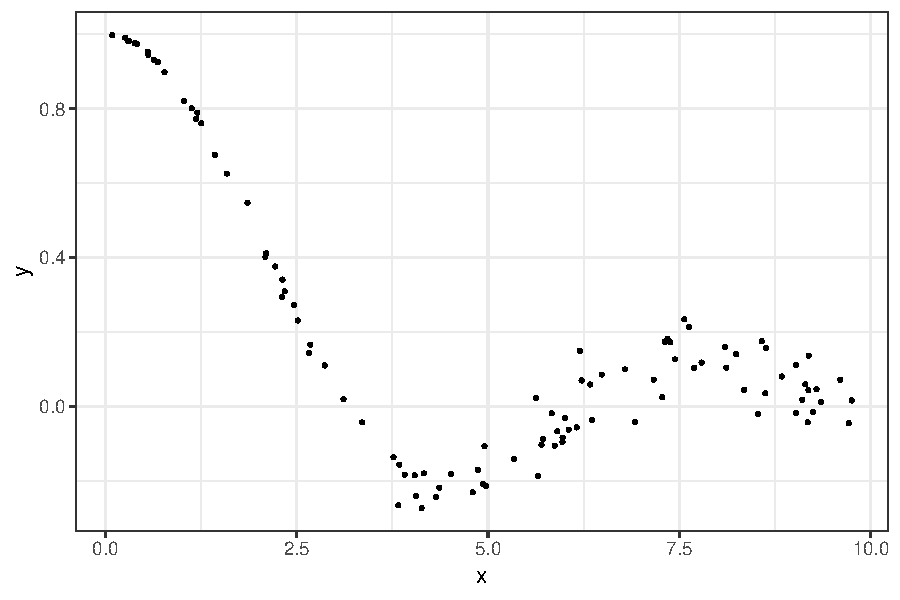
\includegraphics[width=6in]{\detokenize{R/gp_homosked/plots/data.pdf}}
	\caption{$y_i = \sin(x_i) / x_i + \ep_i$; $\ep_i \sim N(0, 0.05)$}
	\label{fig:gphomo:data}
\end{figure}

\end{document}